\documentclass[12pt,a4paper]{article}
\usepackage[utf8]{vietnam}
\usepackage{amsmath,amssymb,amsfonts}
\usepackage[left=2cm,right=2cm,top=2cm,bottom=2cm]{geometry}
\usepackage{tikz}
\usepackage{tkz-tab}
\usetikzlibrary{arrows.meta, calc, intersections}
\usepackage{multicol}
\usepackage{fancyhdr}

% Cấu hình Header & Footer giống file gốc
\pagestyle{fancy}
\fancyhf{}
\lhead{\textbf{Trị Tuyệt Đối 1}}
\rhead{\textbf{TPOC LUYỆN THI TOÁN HSA - 0395339266}}
\cfoot{\thepage}
\renewcommand{\headrulewidth}{0.4pt}

% Định dạng câu hỏi và phương án trắc nghiệm
\newcommand{\cau}[1]{\noindent\textbf{Câu #1. [KMC]} }
\newcommand{\bonpa}[4]{
    \begin{multicols}{4}
        \noindent\textbf{A.} #1
        \par\noindent\textbf{B.} #2
        \par\noindent\textbf{C.} #3
        \par\noindent\textbf{D.} #4
    \end{multicols}
}

\setlength{\parindent}{0pt}
\setlength{\parskip}{6pt}

\begin{document}

% ==================== DẠNG 1 ====================
\section*{DẠNG 1: CỰC TRỊ CỦA HÀM SỐ $y = |f(x)|$ VÀ $y = |f(|x|)|$}

\cau{1} Cho hàm số $f(x)$ có bảng biến thiên như sau:
\begin{center}
\begin{tikzpicture}
    \tkzTabInit[nocadre=true,lgt=1.2,espcl=2.5,deltacl=0.6]
    {$x$ /0.7, $y'$ /0.7, $y$ /2.0}
    {$-\infty$, $-1$, $1$, $+\infty$}
    \tkzTabLine{,+,0,-,0,+,}
    \tkzTabVar{-/$-\infty$, +/$1$, -/$-3$, +/$+\infty$}
\end{tikzpicture}
\end{center}
Hàm số $y = |f(x)|$ có bao nhiêu điểm cực trị?
\bonpa{2.}{3.}{5.}{4.}

\cau{2} Cho hàm số $f(x) = -x^3 + bx^2 + cx + 2$ với $b, c \in \mathbb{R}$. Biết rằng phương trình $f(x) = 0$ có ba nghiệm dương phân biệt. Số điểm cực trị của hàm số $y = |f(|x|)|$ là
\bonpa{9.}{5.}{7.}{11.}

% ==================== DẠNG 2 ====================
\section*{DẠNG 2: CỰC TRỊ CỦA HÀM SỐ $y = f(|x|)$}

\cau{3} Cho hàm số $f(x)$ có đạo hàm $f'(x) = x(x-1)^2(x^2-4), \forall x \in \mathbb{R}$. Số điểm cực trị của hàm số $y = f(|x|)$ là
\bonpa{5.}{3.}{7.}{1.}

\cau{4} Cho hàm số $y = f(x)$ có bảng biến thiên như hình vẽ bên
\begin{center}
\begin{tikzpicture}
    \tkzTabInit[nocadre=true,lgt=1.2,espcl=2.5,deltacl=0.6]
    {$x$ /0.7, $y'$ /0.7, $y$ /2.0}
    {$-\infty$, $-1$, $3$, $+\infty$}
    \tkzTabLine{,+,0,-,0,+,}
    \tkzTabVar{-/$-\infty$, +/$5$, -/$1$, +/$+\infty$}
\end{tikzpicture}
\end{center}
Số điểm cực trị của hàm số $y = f(|x|)$ bằng
\bonpa{5.}{2.}{3.}{4.}

\cau{5} Cho hàm số $f(x)$ có đồ thị như hình vẽ bên. Số điểm cực trị của hàm số $y = f(|x|) + 2023$ là
\begin{center}
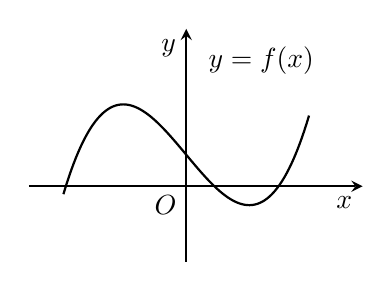
\begin{tikzpicture}[scale=0.8, >=stealth]
    \draw[->, thick] (-2.5,0) -- (2.8,0) node[below left] {$x$};
    \draw[->, thick] (0,-1.2) -- (0,2.5) node[below left] {$y$};
    \node[below left] at (0,0) {$O$};
    \draw[thick, smooth, samples=100, domain=-1.95:1.95] plot(\x, {0.4*(\x)^3 - 1.2*\x + 0.5});
    \node[right] at (0.2, 2.0) {$y=f(x)$};
\end{tikzpicture}
\end{center}
\bonpa{5.}{3.}{2.}{4.}

% ==================== DẠNG 3 ====================
\section*{DẠNG 3: CỰC TRỊ CỦA HÀM SỐ TRỊ TUYỆT ĐỐI CHỨA THAM SỐ $m$}
\subsection*{Nhóm 3.1: Cực trị hàm số $y = f(|x|)$ chứa tham số $m$}

\cau{6} Cho hàm số $f(x) = x^3 - (2m+1)x^2 + (m+2)x + 1$. Có bao nhiêu số nguyên $m \in [-5;5]$ để hàm số $y = f(|x|)$ có đúng ba điểm cực trị.
\bonpa{4.}{6.}{5.}{3.}

\cau{7} Cho hàm số $f(x) = x^3 - (2m+1)x^2 + (m+2)x + 1$. Có bao nhiêu số nguyên $m \in [-5;5]$ để hàm số $y = f(|x|)$ có 5 điểm cực trị?
\bonpa{4.}{6.}{5.}{3.}

\cau{8} Cho hàm số $f(x) = (m-1)x^3 - 5x^2 + (m+3)x + 3$. Tìm tất cả các giá trị nguyên của tham số $m$ để hàm số $y = f(|x|)$ có đúng 3 điểm cực trị?

\cau{9} Cho hàm số $y = f(x) = x^3 - (2m-1)x^2 + (2-m)x + 2$. Tìm tất cả các giá trị của $m$ để đồ thị hàm số $y = f(|x|)$ có 5 điểm cực trị.

\subsection*{Nhóm 3.2: Cực trị hàm số $y = |f(x,m)|$ chứa tham số $m$}

\cau{10} Tìm tất cả các giá trị thực của tham số $m$ để hàm số $y = |x^3 - 3x^2 + m|$ có 5 điểm cực trị.
\bonpa{$-4 < m < 0$.}{$-4 \le m \le 0$.}{$0 < m < 4$.}{$m \ge 4$ hoặc $m \le 0$.}

\cau{11} Cho hàm số $y = f(x)$ có bảng biến thiên như hình vẽ:
\begin{center}
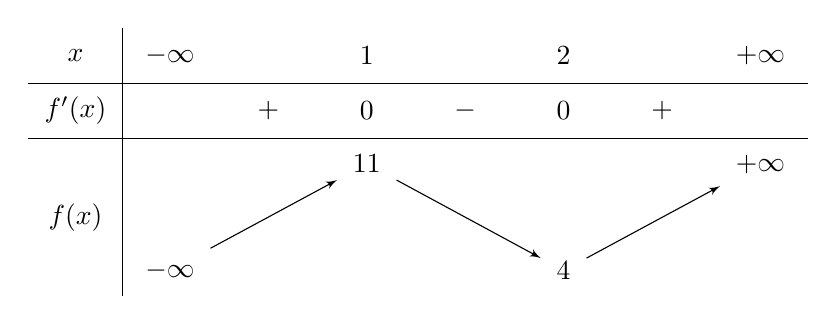
\begin{tikzpicture}
    \tkzTabInit[nocadre=true,lgt=1.2,espcl=2.5,deltacl=0.6]
    {$x$ /0.7, $f'(x)$ /0.7, $f(x)$ /2.0}
    {$-\infty$, $1$, $2$, $+\infty$}
    \tkzTabLine{,+,0,-,0,+,}
    \tkzTabVar{-/$-\infty$, +/$11$, -/$4$, +/$+\infty$}
\end{tikzpicture}
\end{center}
Đồ thị hàm số $y = |f(x) - 2m|$ có 5 điểm cực trị khi và chỉ khi
\bonpa{$m \in (4;11)$.}{$m \in \left(2; \dfrac{11}{2}\right)$.}{$m = 3$.}{$m \in \left[2; \dfrac{11}{2}\right]$.}

\cau{12} Cho hàm bậc ba $y = f(x)$ có đồ thị như hình vẽ bên. Tất cả các giá trị thực của tham số $m$ để hàm số $y = |f(x) + m|$ có 5 điểm cực trị là
\begin{center}
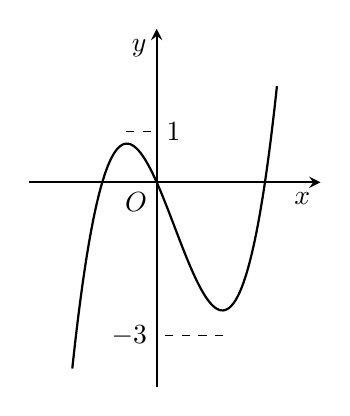
\begin{tikzpicture}[scale=0.65, >=stealth]
    \draw[->, thick] (-2.5,0) -- (3.2,0) node[below left] {$x$};
    \draw[->, thick] (0,-4) -- (0,3) node[below left] {$y$};
    \node[below left] at (0,0) {$O$};
    \draw[thick, smooth, samples=100, domain=-1.65:2.35] plot(\x, {(\x)^3 - 1.05*(\x)^2 - 2.25*\x});
    \draw[dashed] (-0.6, 1) -- (0, 1) node[right] {$1$};
    \draw[dashed] (1.3, -3) -- (0, -3) node[left] {$-3$};
\end{tikzpicture}
\end{center}
\bonpa{$m \le -1$ hoặc $m \ge 3$.}{$-1 < m < 3$.}{$m = -1$ hoặc $m = 3$.}{$1 < m < 3$.}

\cau{13} Cho hàm số $f(x)$ có bảng biến thiên như sau:
\begin{center}
\begin{tikzpicture}
    \tkzTabInit[nocadre=true,lgt=1.2,espcl=2.5,deltacl=0.6]
    {$x$ /0.7, $y'$ /0.7, $y$ /2.0}
    {$-\infty$, $-1$, $1$, $+\infty$}
    \tkzTabLine{,+,0,-,0,+,}
    \tkzTabVar{-/$-\infty$, +/$1$, -/$-3$, +/$+\infty$}
\end{tikzpicture}
\end{center}
Có bao nhiêu số nguyên $m$ để hàm số $y = |f(x) + m|$ có 5 điểm cực trị?
\bonpa{5.}{6.}{3.}{4.}

\cau{14} Có bao nhiêu số nguyên $m$ để hàm số $y = |3x^4 - 4x^3 - 12x^2 + m|$ có 7 điểm cực trị
\bonpa{3.}{5.}{6.}{4.}

\cau{15} Có tất cả bao nhiêu giá trị nguyên dương của tham số $m$ để hàm số $y = |3x^4 - 4x^3 - 12x^2 + m|$ có đúng 5 điểm cực trị?
\bonpa{16.}{28.}{26.}{27.}

\cau{16} Cho hàm số $f(x) = |x^3 + (m+2)x^2 + mx - m^2|$. Có bao nhiêu giá trị nguyên của $m$ thoả mãn $|m-1| < 5$ để hàm số đã cho có đúng 5 điểm cực trị?
\bonpa{6.}{3.}{5.}{4.}

\cau{17} Gọi $S$ là tập hợp các giá trị nguyên của $m$ để hàm số $y = |x^5 - 5x^3 + 5x^2 + 3m - 7|$ có 5 điểm cực trị. Tổng các phần tử của $S$ bằng
\bonpa{16.}{$-16$.}{18.}{$-18$.}

% ==================== DẠNG 4 ====================
\section*{DẠNG 4: TÍNH ĐƠN ĐIỆU CỦA HÀM SỐ TRỊ TUYỆT ĐỐI CHỨA THAM SỐ}

\cau{18} Có bao nhiêu giá trị nguyên dương của tham số $m$ để hàm số $y = |x^3 - 3x^2 + m|$ đồng biến trên khoảng $(1;2)$?
\bonpa{2.}{Vô số.}{3.}{1.}

\cau{19} Cho hàm số $f(x) = x^3 - (2m-1)x^2 + (2-m)x + 2$. Tìm tập hợp giá trị thực của tham số $m$ để hàm số $y = f(|x|)$ có năm điểm cực trị.
\bonpa{$-\dfrac{5}{4} < m < 2$.}{$\dfrac{5}{4} < m < 2$.}{$\dfrac{1}{2} < m < 2$.}{$-2 < m < \dfrac{5}{4}$.}

\cau{20} Tìm tất cả các giá trị thực của tham số $m$ để hàm số $y = |x|^3 - (2m+1)x^2 + 3m|x| - 5$ có đúng 3 điểm cực trị.
\bonpa{$(-\infty; 0)$.}{$(1; +\infty)$.}{$(-\infty; 0]$.}{$\left[0; \dfrac{1}{4}\right)$.}

\cau{21} Có bao nhiêu số nguyên $m \in (-20;20)$ để hàm số $y = \left|\dfrac{1}{3}x^3 - x^2 + (m^2+2)x + m\cdot\cos x\right|$ đồng biến trên khoảng $(0;\pi)$?
\bonpa{33.}{32.}{19.}{20.}

\cau{22} Có bao nhiêu giá trị nguyên của tham số $a \in (-10; +\infty)$ để hàm số $y = |x^3 + (a+2)x + 9 - a^2|$ đồng biến trên khoảng $(0;1)$?
\bonpa{12.}{11.}{6.}{5.}

\cau{23} Có bao nhiêu số tự nhiên $m$ để hàm số $f(x) = |\sin^3 x - m\sin x + 1|$ đồng biến trên khoảng $\left(0; \dfrac{\pi}{2}\right)$?
\bonpa{1.}{3.}{2.}{0.}

\cau{24} Cho hàm số $f(x)$ có đạo hàm trên $\mathbb{R}$ và $f(1) = 1$. Đồ thị hàm số $y = f'(x)$ như hình bên. Có bao nhiêu số nguyên dương $a$ để hàm số $y = |4f(\sin x) + \cos 2x - a|$ nghịch biến trên $\left(0; \dfrac{\pi}{2}\right)$?
\begin{center}
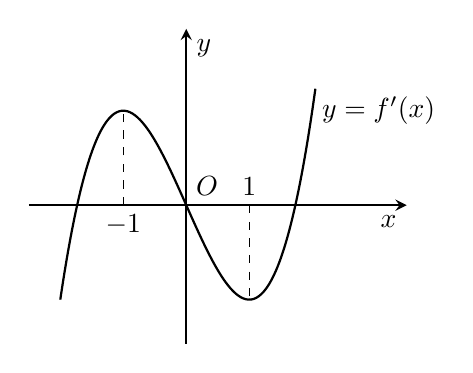
\begin{tikzpicture}[scale=0.8, >=stealth]
    \draw[->, thick] (-2.5,0) -- (3.5,0) node[below left] {$x$};
    \draw[->, thick] (0,-2.2) -- (0,2.8) node[below right] {$y$};
    \node[above right] at (0,0) {$O$};
    \draw[thick, smooth, samples=100, domain=-2.0:2.05] plot(\x, {0.75*(\x)^3 - 2.25*\x});
    \draw[dashed] (-1,0) node[below] {$-1$} -- (-1,1.5);
    \draw[dashed] (1,0) node[above] {$1$} -- (1,-1.5);
    \node[right] at (2.0, 1.5) {$y=f'(x)$};
\end{tikzpicture}
\end{center}
\bonpa{2.}{3.}{Vô số.}{5.}

\cau{25} Có bao nhiêu giá trị nguyên của $a$ sao cho hàm số $y = |x^3 - 3x^2 - ax + a|$ đồng biến trên khoảng $(0; +\infty)$?
\bonpa{Vô số.}{2.}{0.}{1.}

\cau{26} Có bao nhiêu cặp số nguyên $(m;n)$ với $m, n \in [-5;5]$ để hàm số $f(x) = |x^3 - 3x^2 + mx + n|$ đồng biến trên $(0; +\infty)$?
\bonpa{15.}{24.}{18.}{25.}

\cau{27} Có bao nhiêu số tự nhiên $m$ để hàm số $y = |x^4 - mx + 1|$ đồng biến trên khoảng $(1; +\infty)$.
\bonpa{3.}{2.}{4.}{5.}

\cau{28} Có bao nhiêu số nguyên $m \in [-9;9]$ để hàm số $f(x) = \left|-\dfrac{1}{3}x^3 + \dfrac{1}{2}(2m+3)x^2 - (m^2+3m)x + \dfrac{2}{3}\right|$ nghịch biến trên khoảng $(1;2)$?
\bonpa{2.}{16.}{3.}{19.}

\cau{29} Cho hàm số $f(x)$ liên tục trên $\mathbb{R}$ có $f(2) = 1$ và đồ thị hàm số $f'(x)$ như hình vẽ bên:
\begin{center}
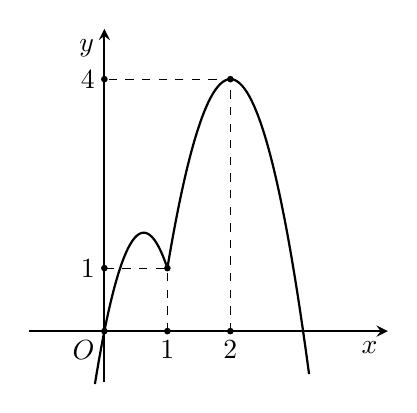
\begin{tikzpicture}[scale=0.8, >=stealth]
    \draw[->, thick] (-1.2,0) -- (4.5,0) node[below left] {$x$};
    \draw[->, thick] (0,-0.8) -- (0,4.8) node[below left] {$y$};
    \node[below left] at (0,0) {$O$};
    \draw[thick, smooth, samples=100, domain=-0.15:1] plot(\x, {-4*(\x)^2 + 5*\x});
    \draw[thick, smooth, samples=100, domain=1:3.25] plot(\x, {-3*(\x-2)^2 + 4});
    \draw[dashed] (1,0) node[below] {$1$} -- (1,1) -- (0,1) node[left] {$1$};
    \draw[dashed] (2,0) node[below] {$2$} -- (2,4) -- (0,4) node[left] {$4$};
    \fill (0,0) circle (1.5pt) (1,0) circle (1.5pt) (2,0) circle (1.5pt) (0,1) circle (1.5pt) (0,4) circle (1.5pt) (1,1) circle (1.5pt) (2,4) circle (1.5pt);
\end{tikzpicture}
\end{center}
Có bao nhiêu số nguyên dương $a$ để hàm số $y = |3f(x) - x^3 + a|$ nghịch biến trên khoảng $(0;2)$?
\bonpa{3.}{5.}{6.}{4.}

\cau{30} Số giá trị nguyên của tham số $m$ để hàm số $y = |x^3 + (2m-2)x + 16 - m^2|$ đồng biến trên $(0; +\infty)$ là
\bonpa{2.}{3.}{1.}{4.}

\cau{31} Có bao nhiêu số nguyên $m$ để hàm số $y = |x-m| + |x+m+2|$ đồng biến trên khoảng $(0; +\infty)$.
\bonpa{3.}{1.}{4.}{Vô số.}

\cau{32} Có bao nhiêu số nguyên $m$ để hàm số $y = |x-m| + |x+m+2|$ nghịch biến trên khoảng $(-\infty; -3)$.
\bonpa{3.}{5.}{4.}{Vô số.}

\cau{33} Có bao nhiêu giá trị nguyên của tham số $m \in [-20;20]$ để hàm số $y = |x^2 - mx + 4| - x^2 + 4x$ đồng biến trên khoảng $(1;4)$?
\bonpa{34.}{33.}{32.}{35.}

% ==================== DẠNG 5 ====================
\section*{DẠNG 5: GIÁ TRỊ LỚN NHẤT - GIÁ TRỊ NHỎ NHẤT CỦA HÀM SỐ TRỊ TUYỆT ĐỐI CHỨA THAM SỐ $m$}

\cau{34} Có bao nhiêu số thực $m$ để hàm số $y = |3x^4 - 4x^3 - 12x^2 + m|$ có giá trị lớn nhất trên đoạn $[-3;2]$ bằng $150$.
\bonpa{4.}{0.}{2.}{6.}

\cau{35} Có bao nhiêu số thực $m$ để hàm số $y = |3x^4 - 4x^3 - 12x^2 + m|$ có giá trị lớn nhất trên đoạn $[-3;2]$ bằng $\dfrac{275}{2}$.
\bonpa{4.}{0.}{2.}{1.}

\cau{36} Có bao nhiêu số thực $m$ để hàm số $y = |3x^4 - 4x^3 - 12x^2 + m|$ có giá trị lớn nhất trên đoạn $[-3;2]$ bằng $136$.
\bonpa{4.}{0.}{2.}{1.}

\cau{37} Giá trị lớn nhất của hàm số $y = |3x^4 - 4x^3 - 12x^2 + m|$ trên đoạn $[-3;2]$ có giá trị nhỏ nhất bằng
\bonpa{$\dfrac{211}{2}$.}{$\dfrac{275}{2}$.}{$\dfrac{137}{2}$.}{$\dfrac{115}{2}$.}

\cau{38} Cho hàm số $y = |x^2 + x + m|$. Tổng tất cả các giá trị thực của tham số $m$ sao cho $\min_{[-2;2]} y = 2$ bằng
\bonpa{$-\dfrac{31}{4}$.}{$-8$.}{$-\dfrac{23}{4}$.}{$\dfrac{9}{4}$.}

\cau{39} Cho hàm số $y = \left|\dfrac{x - m^2 - m}{x+2}\right|$. Có bao nhiêu giá trị thực của tham số $m$ để $\max_{[1;2]} y = 1$.
\bonpa{4.}{2.}{3.}{1.}

\cau{40} Cho hàm số $y = \left|\dfrac{x - m^2 - m}{x+2}\right|$. Giá trị lớn nhất của hàm số trên đoạn $[1;2]$ có giá trị nhỏ nhất bằng
\bonpa{$\dfrac{1}{6}$.}{}{}{}

\cau{41} Cho hàm số $y = \left|\dfrac{x - m^2 + m}{x+1}\right|$. Giá trị lớn nhất của hàm số trên đoạn $[1;2]$ có giá trị nhỏ nhất bằng
\bonpa{$\dfrac{1}{7}$.}{}{}{}

\end{document}